\newcommand\obseq{\stackrel{\sim}{=}}
\newcommand\CS{\{c,\sigma\}}
\newcommand\CpSp{\{c',\sigma'\}}
\newcommand\numCS[1]{\{c_{#1},\sigma_{#1}\}}


% \begin{figure*}
% \centering
% 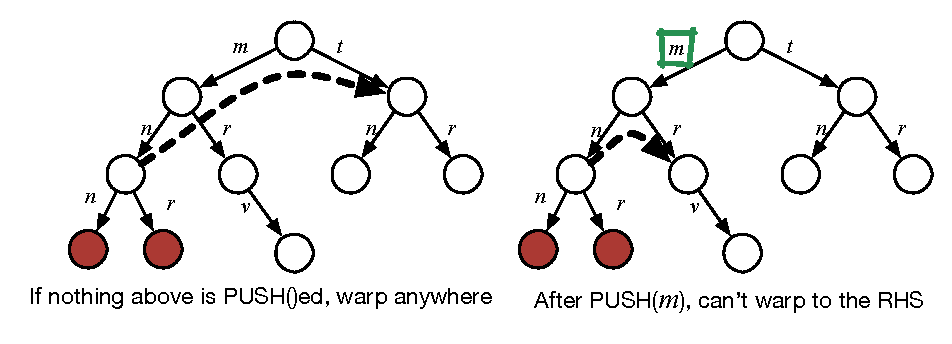
\includegraphics[width=5in]{stages.eps}
% \caption{\red{caption.}}
% \end{figure*}
\begin{figure}
\figbox{
$$
\infer{  \step{c_1 \semit c_2}{m}{c' \semit c_2} }
      {  \step{c_1}{m}{c'} }
\hspace{0.07in}
\infer{  \step{c_1 \semit c_2}{m}{c} }
      {  \nothing{c_1} & \step{c_2}{m}{c} }
\hspace{0.07in}
\infer{  \step{(c)^*}{m}{c'} }
      {  \step{c \semit (c)^*}{m}{c'} }
$$
$$
\infer{  \step{c_1 \plust c_2}{m}{c} }
      {  \step{c_1}{m}{c} }
\qquad
\infer{  \step{c_1 \plust c_2}{m}{c} }
      {  \step{c_2}{m}{c} }
\qquad
\infer{  \step{m}{m}{\skipt} }{}
$$

$$
\infer{  \nothing{c_1 \semit c_2} }
      {  \nothing{c_1} 
      &  \nothing{c_2} }
\qquad
\infer{  \nothing{c_1 \plust c_2} }
      {  \nothing{c_1} }
\qquad
\infer{  \nothing{c_1 \plust c_2} }
      {  \nothing{c_2} }
\qquad
\infer{ \nothing{\skipt} }{}
$$
\red{do looping fin rule.}
}
\caption{Reduction semantics 
$\step{c}{m}{c'}$ and $\nothing{c}$
for the example language.}
\end{figure}

\section{Technical Background}

In this section we provide the technical background for our work,
including preliminary definitions and a brief summary of the \PMPY{}
model of tarnsactions~\cite{KP:PLDI15}.

\subsection{Preliminaries and atomic semantics}

% We first describe a generic language of transactions and
% define an idealized semantics for concurrent transactions called the
% atomic semantics, in which there are no interleaved effects on the
% shared state. 
%
%The model preliminaries generalize those provided previously~\cite{PMPY}.
%
%We also define a notion of \emph{good} configurations
%and in the next section we will define how one can warp from a 
%configuraiton that is not good to one that is.

\paragraph{Operations and States.}
We assume a set $M$ of method calls or operations (\eg\
  \texttt{ht.put('a',5)}).
%
State is represented in terms of
logs of operation records. An operation record (or, simply, an ``operation'')
$
    \op = \langle \opname, \lstack_1, \lstack_2, \opid \rangle
$
is a tuple consisting of the operation name $m$, 
a thread-local pre-stack $\lstack_1$ (method arguments),
a thread-local post-stack $\lstack_2$ (method return values),
and a unique identifier $\opid$.
%
We assume a predicate $\fresh{\opid}$ that holds provided that $\opid$
is globally unique (details omitted for lack of space).
%
In the atomic semantics defined below, the shared state $\OPL :
\textsf{list } \op$ is an ordered list of operations.
%
We use notations such as $\OPL_1\cdot\OPL_2$ and $\OPL\cdot \op$ to
mean append and appending a singleton, resp.

%\begin{parameter}[From logs to states: $\allowedt{}$] 
We require a prefix-closed predicate on operation lists $\allowed{\OPL}$
that indicates whether an operation log $\OPL$ corresponds to a state.
% The sequential specification
%   is a predicate on operation lists: $\allowed{\OPL}$. We require that it
%   be prefix closed.
%\end{parameter}
%
%\noindent
For convenience we will also write $\OPL \allows \langle m, \lstack_1,
\lstack_2, \opid\rangle$ which simply means 
$\allowed{\OPL \cdot \langle m, \lstack_1,\lstack_2, \opid\rangle}$.
%
For example, if we have a simple TM
based on memory read/write operations we expect
$\;\;\allowed{\OPL\cdot \langle \texttt{a := x}, [x \mapsto 5], [x
  \mapsto 5, a \mapsto 5], \opid\rangle}$,
but 
$\;\;\neg \allowed{\OPL\cdot \langle \texttt{a := x}, [x \mapsto 5], [x
  \mapsto 5, a \mapsto 3], \opid\rangle}$ or more elaborate
specifications that involve multiple tasks.
%
Ultimately, we expect the $\allowed{}$ predicate to be induced by the
implementation's operations on the state, $\llbracket op\rrbracket :
\mathcal{P}(\mathsf{State} \times \mathsf{State})$, and initial
states $I$. 
% If we give a denotation to logs as $\llbracket \OPL \cdot op
% \rrbracket \equiv \llbracket \OPL \rrbracket ; \llbracket op
% \rrbracket$, and $\llbracket \epsilon \rrbracket \equiv I$ , where $
% S ; R \equiv \{ s' \mid \exists s \in S. (s,s') \in R \}$. Then we
% can define $\allowed{\OPL}$ simply by checking if the denotation is
% non-empty, $(\llbracket \OPL \rrbracket \neq \emptyset)$.

%\paragraph{Operational equivalence.}
We define a precongruence over operation logs $\OPL_1 \opeq \OPL_2$
coinductively, by requiring that all \allowedt\ extensions of the log $\OPL_1$, are also \allowedt\ extension to the log $\OPL_2$. 
% This definition will ultimately be used in the simulation between
% \PMPY{} and an atomic machine.
We use a coinductive definition so that the precongruence can be
defined up to all infinite suffixes.
%\begin{definition}[Shared log precongruence $\opeq$] For all $\OPL_1, \OPL_2$,
$$
\infer={\OPL_1 \opeq \OPL_2} 
%   {\deduce{\allowed{\OPL_1}}  {\allowed{\OPL_2}}
   {  \allowed{\OPL_1} \Rightarrow \allowed{\OPL_2}
     & \forall \op.\   (\OPL_1 \cdot \op) \opeq (\OPL_2 \cdot \op)}
$$
We use a double-line here to indicate greatest fixpoint.
%\end{definition}
%
Informally, the above definition says that 
there is no sequence of observations we can make of $\OPL_2$, that we can't also make of $\OPL_1$. 
This is more general than just considering the set of states reached from executing the first log is included in the second:
unobservable state differences are also permitted. 


\paragraph{Language.}

For the sake of presentation, let us
say that the code is given by the following language 
\[ \begin{array}{rcl}
  c &::=& c_1\plust c_2 \MOR c_1 \semit c_2
      \MOR (c)^* \MOR \skipt \MOR \tx{c} \MOR \opname
\end{array} \]
This grammar additionally consists of nondeterministic choice, sequential
composition, and nondeterministic looping.
%,  \skipt, a transaction $\tx{c}$, and operations denoted $\opname$.
As done elsewhere~\cite{KP:PLDI15}, we abstract away the programming
language with a few semantic functions: \red{update this with pldi
  camera ready}
%
\begin{description}
\item[$\step{c}{m}{c'}$:] Within a transaction, code $c$ can be reduced to the pair
  $(m,c')$.  That is, $m$ is a next reachable method call in the
  reduction of $c$, with remaining code $c'$.

\item[$\tstep{c}{t}{c'}$:] Outside of a transaction, code $c$ can be reduced to the pair
  $(t,c')$.  Here $c'$ is the remaining code, and $t$ is either
  a local state update, or a transaction or a thread fork.

\item[$\nothing{c}$:] This predicate is true provided that there is a
  reduction of $c$ to $\skipt$ that does not encounter a method call.
\end{description}
%
These functions allow us to obtain a simple semantics, despite an
expressive input language, by introducing functions to resolve
nondeterminism between method operation names and at the end of a
transaction.
%  As an example, one might use the generic language:
% \[ \begin{array}{rcl}
%   c &::=& c_1\plust c_2 \MOR c_1 \semit c_2
%       \MOR (c)^* \MOR \skipt \MOR \tx{c} \MOR \opname
% \end{array} \]
% %
% which consists of nondeterministic choice, sequential
% composition, and nondeterministic looping.
%
We assume that code is well-formed in that a single operation name $\opname$ 
is always contained within a transaction. 


The rules for $\step{c}{m}{c'}$ and $\nothing{c}$ are given in
Figure~\ref{fig:stepfin}.
\red{explain}
For example, if 
$
c \;=\; \tx{(\skipt \semit (c_1 \plust (m \plust n)) \semit c_2)}
$,
then one path through $c$ reaches method $n$ with a continuation of $c_2$. Hence,
$ \step{c}{n}{c_2}$.


% Threads execute code $c$ from some programming language that
% includes thread forking, transactions $\tx{c}$,
% method names such as $m$, and a \skipt\ statement.


The atomic semantics $\xrightarrow{a}$,
in which transactions are executed instantly, without interruption
from concurrent threads is given in Appendix~\ref{apx:atomic}.
Threads in the atomic semantics are represented as a pair
$(c,\sigma)$ of the code $c$ and a small amount of local
information $\sigma$ used to model arguments and return values.


%%% Local Variables:
%%% mode: latex
%%% TeX-master: "paper"
%%% End:
